% ========================================
% ROTATIONAL TRANSFORMATIONS
% ========================================

% Frame 1: 2D Rotation Visualization
\begin{frame}{Rotation Transformations in $\mathbb{R}^2$}
    \begin{itemize}
        \item \textbf{Two-dimensional rotation:}
    \end{itemize}
    
    \begin{figure}[h]
        \centering
        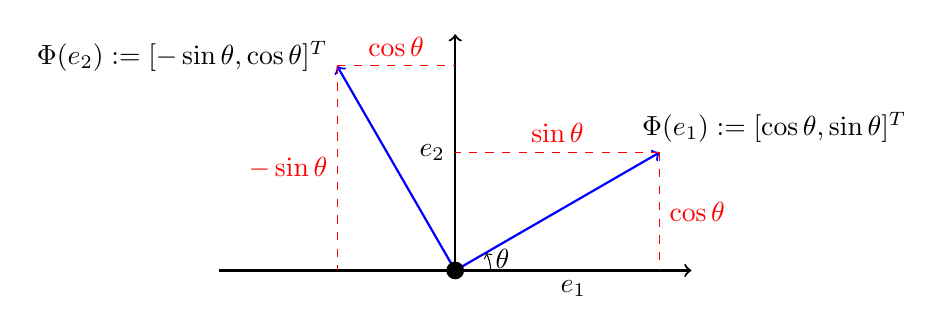
\begin{tikzpicture}[scale=1.5]
            % Origin
            \coordinate (O) at (0,0);
            \coordinate (OO) at (-2,0);

            % Standard basis vectors
            \draw[->, thick] (O) -- (2,0) node[midway, below] {$e_1$};
            \draw[->, thick] (OO) -- (O) -- (0,2) node[midway, left] {$e_2$};

            % Rotated basis vectors
            \draw[->, thick, blue] (O) -- ({2*cos(30)}, {2*sin(30)});
            \node at (1.5, 1) [above right] {$\Phi(e_1) := [\cos \theta, \sin \theta]^T$};
            \draw[->, thick, blue] (O) -- ({2*-sin(30)}, {2*cos(30)});
            \node at (-1, 1.6) [above left] {$\Phi(e_2) := [-\sin \theta, \cos \theta]^T$};

            % Reference lines
            \draw[dashed, red] ({2*cos(30)}, {2*sin(30)}) -- ({2*cos(30)}, 0) node[midway, right] {$\cos \theta$};
            \draw[dashed, red] ({2*-sin(30)}, {2*cos(30)}) -- (0, {2*cos(30)}) node[midway, above] {$\cos \theta$};
            \draw[dashed, red] ({2*-sin(30)}, {2*cos(30)}) -- ({2*-sin(30)}, 0) node[midway, left] {$- \sin \theta$};
            \draw[dashed, red] ({2*cos(30)}, {2*sin(30)}) -- (0, {2*sin(30)}) node[midway, above] {$\sin \theta$};

            % Origin marker
            \filldraw[black] (O) circle (2pt);
            
            % Rotation angle
            \draw[->] (0.3,0) arc[start angle=0, end angle=30, radius=0.3];
            \node at (0.4, 0.1) {$\theta$};
        \end{tikzpicture}
        \caption{Standard basis rotation in $\mathbb{R}^2$ through angle $\theta$}
        \label{fig:rotation_2d_basis}
    \end{figure}
\end{frame}

% Frame 2: 2D Rotation Matrix
\begin{frame}{Matrix Representation of 2D Rotation}
    \begin{itemize}
        \item \textbf{Derivation:} From the transformed basis vectors in the previous slide:
        \begin{align}
            \Phi(e_1) &= \begin{bmatrix} \cos \theta \\ \sin \theta \end{bmatrix}, \quad
            \Phi(e_2) = \begin{bmatrix} -\sin \theta \\ \cos \theta \end{bmatrix}
        \end{align}
        
        \item The rotation transformation matrix $R_\theta$ has these as columns:
        \begin{align}
            R_\theta = \begin{bmatrix}
                \cos \theta & -\sin \theta \\
                \sin \theta & \cos \theta
            \end{bmatrix}
        \end{align}
    \end{itemize}
\end{frame}
\begin{frame}
    \begin{itemize}
        \item Given a vector $\mathbf{x}$, its rotation by angle $\theta$ yields $\mathbf{y}$:
        \begin{align}
            \mathbf{y} = \begin{bmatrix}
                y_1 \\
                y_2
            \end{bmatrix} = \begin{bmatrix}
                \cos \theta & -\sin \theta \\
                \sin \theta & \cos \theta
            \end{bmatrix} \begin{bmatrix}
                x_1 \\
                x_2
            \end{bmatrix}
        \end{align}
    \end{itemize}
\end{frame}

% Frame 3: 3D Rotation Visualization
\begin{frame}{Rotation Transformations in $\mathbb{R}^3$}
    \begin{figure}[h]
        \centering
        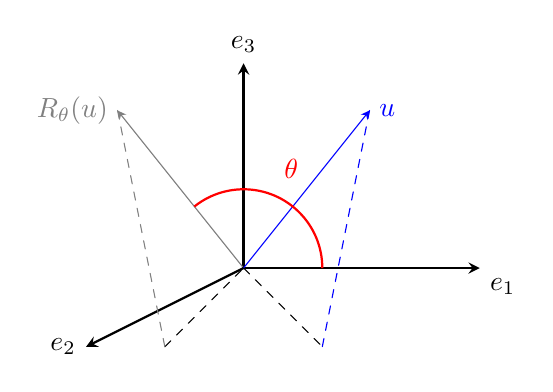
\begin{tikzpicture}[scale=2.0, line cap=round, line join=round, >=stealth]
            % Coordinate points
            \coordinate (O) at (0,0);
            \coordinate (E1) at (1.5, 0);
            \coordinate (E3) at (0, 1.3);
            \coordinate (E2) at (-0.8, 1.0);
            \coordinate (E4) at (0.8, 1.0);
            
            % Coordinate axes
            \draw[->, thick] (O) -- (E1) node[below right] {$e_1$};
            \draw[->, thick] (O) -- (E3) node[above] {$e_3$};
            \draw[->, gray] (O) -- (E2) node[left] {$R_{\theta}(u)$};
            \draw[dashed] (-.5,-.5) -- (O);
            \draw[->, thick] (O) -- (-1,-.5) node[left] {$e_2$};
            \draw[->, blue] (O) -- (E4) node[right] {$u$};
            \draw[dashed,gray] (E2) -- (-.5,-.5);
            \draw[dashed, blue] (E4) -- (.5, -.5);
            \draw[dashed] (O) -- (.5, -.5);
            
            % Rotation angle arc
            \pgfmathsetmacro{\angEtwo}{atan2(1.0, -0.8)}
            \begin{scope}
                \clip (O) -- (E1) -- (E2);
                \draw[red, thick] (0.5, 0) arc[start angle=0, end angle=\angEtwo, radius=0.5];
            \end{scope}
            \node[red] at (\angEtwo/2:0.7) {$\theta$};
        \end{tikzpicture}
        \caption{Vector rotation in $\mathbb{R}^3$ around the $e_3$-axis by angle $\theta$}
        \label{fig:rotation_3d}
    \end{figure}
\end{frame}

% Frame 4: 3D Rotation Matrices (Part 1)
\begin{frame}{Rotation Matrices in Three Dimensions}
    \begin{itemize}
        \item \textbf{Rotation around the $e_1$-axis:}
        \begin{align}
            R_1(\theta) = \begin{bmatrix}
                1 & 0 & 0 \\
                0 & \cos \theta & -\sin \theta \\
                0 & \sin \theta & \cos \theta
            \end{bmatrix}
        \end{align}
        
        \item \textbf{Rotation around the $e_2$-axis:}
        \begin{align}
            R_2(\theta) = \begin{bmatrix}
                \cos \theta & 0 & \sin \theta \\
                0 & 1 & 0 \\
                -\sin \theta & 0 & \cos \theta
            \end{bmatrix}
        \end{align}
    \end{itemize}
\end{frame}

% Frame 5: 3D Rotation Matrices (Part 2) and Properties
\begin{frame}{Additional 3D Rotation Matrix and Key Properties}
    \begin{itemize}
        \item \textbf{Rotation around the $e_3$-axis:}
        \begin{align}
            R_3(\theta) = \begin{bmatrix}
                \cos \theta & -\sin \theta & 0 \\
                \sin \theta & \cos \theta & 0 \\
                0 & 0 & 1
            \end{bmatrix}
        \end{align}
        
        \item In each rotation, the corresponding axis $e_i$ remains invariant.
    \end{itemize}
\end{frame}

% Frame 6: Problem Set
\begin{frame}{Exercises on Rotation Matrices}
    \textbf{Problem:} Demonstrate the following fundamental properties of rotation matrices:
    \begin{enumerate}
        \item Distance preservation: For any angle $\theta$, verify that:
        $$\|\mathbf{x} - \mathbf{y}\| = \|R_\theta(\mathbf{x}) - R_\theta(\mathbf{y})\|$$
        holds for all vectors $\mathbf{x}, \mathbf{y}$.
        
        \item Rotation composition: Prove that $R_{\theta + \phi} = R_{\theta} \cdot R_{\phi}$ for all $\theta, \phi \in [0, 2\pi)$.
    \end{enumerate}
\end{frame}

\begin{frame}
    \begin{itemize}
        \item Identity and inverse relations: Establish that $R_{0} = I$ and $R_{-\theta} = R_{\theta}^{-1}$.
        
        \item Angular preservation: Demonstrate that rotations maintain inner products:
        $$\langle R_\theta \mathbf{x}, R_\theta \mathbf{y} \rangle = \langle \mathbf{x}, \mathbf{y} \rangle$$
        for all vectors $\mathbf{x}, \mathbf{y}$.
    \end{itemize}
\end{frame}

\begin{frame}
    \textbf{Exercise:} Consider the rotation matrix $R_\theta$ defined as:
    \begin{align}
        R_\theta = \begin{bmatrix}
            \cos \theta & -\sin \theta \\
            \sin \theta & \cos \theta
        \end{bmatrix}
    \end{align}
    \begin{itemize}
        \item Show that $R_\theta$ is orthogonal, i.e., $R_\theta^T R_\theta = I$.
        \item Verify that the determinant of $R_\theta$ is 1, confirming that it represents a rotation.
        \item Prove that the inverse of $R_\theta$ is its transpose, i.e., $R_\theta^{-1} = R_\theta^T$.
    \end{itemize}
\end{frame}

\begin{frame}
    \textbf{Exercise:} Given a vector $\mathbf{x} = \begin{bmatrix} x_1 \\ x_2 \end{bmatrix}$, compute its rotation by angle $\theta$ using the matrix $R_\theta$:
    \begin{align}
        \mathbf{y} = R_\theta \mathbf{x} = \begin{bmatrix}
            \cos \theta & -\sin \theta \\
            \sin \theta & \cos \theta
        \end{bmatrix} \begin{bmatrix}
            x_1 \\
            x_2
        \end{bmatrix}
    \end{align}
    \begin{itemize}
        \item Calculate the resulting vector $\mathbf{y}$.
        \item Discuss how the rotation affects the coordinates of $\mathbf{x}$.
    \end{itemize}   
\end{frame}
\begin{frame}
    \textbf{Exercise:} Consider the rotation matrix $R_\theta$ and a vector $\mathbf{x} = \begin{bmatrix} x_1 \\ x_2 \end{bmatrix}$.
    \begin{itemize}
        \item Compute the rotated vector $\mathbf{y} = R_\theta \mathbf{x}$.
        \item Verify that the angle between $\mathbf{x}$ and $\mathbf{y}$ is $\theta$.
        \item Discuss the geometric interpretation of this rotation in the context of the standard basis vectors.
    \end{itemize}
\end{frame}
